% =============================================================================
% File:  data_management.tex -- 
% Author(s): Sebastien Varrette (sebastien.varrette@uni.lu)
% Time-stamp: <Mon 2015-06-29 17:18 svarrette>
% 
% Copyright (c) 2015 Sebastien Varrette<Sebastien.Varrette@uni.lu>
% 
% For more information:
% - LaTeX: http://www.latex-project.org/
% - Beamer: https://bitbucket.org/rivanvx/beamer/
% - LaTeX symbol list:
% http://www.ctan.org/tex-archive/info/symbols/comprehensive/symbols-a4.pdf
% =============================================================================

\documentclass[t]{beamer}
% \documentclass[draft]{beamer}
\usepackage{_style}

% The key part to use my theme -- if you precise nothing, the image that
% illustrate the slides is assumed to be images/slides_image.jpg
\usetheme[image=images/logo_ULHPC.pdf]{Falkor}

% Not integrated in my theme as not everybody wants that
\AtBeginSection[]
{
  \frame{
    \frametitle{Summary}
    {\scriptsize\tableofcontents[currentsection]}
  }
}

\graphicspath{{logos/}{images/}} % Add this directory to the searched paths for graphics


\newcommand{\bbegin}[1]{\begin{block}{#1}}
\newcommand{\bend}{\end{block}}
\newcommand{\exbegin}[1]{\begin{exampleblock}{#1}}
\newcommand{\exend}{\end{exampleblock}}
\newcommand{\wbegin}[1]{\begin{alertblock}{#1}}
\newcommand{\wend}{\end{alertblock}}
\newcommand{\warn}[2]{\begin{alertblock}{#1}#2\end{alertblock}}
\newcommand{\ex}[2]{\begin{exampleblock}{#1}#2\end{exampleblock}}
\newcommand{\toyou}[1]{\ex{}{\centering Your Turn! #1}}
\newcommand{\command}[1]{\begin{tcolorbox}[colback=black!5!white,colframe=white!75!black,leftrule=3mm]\cmdlineentry{\scriptsize #1}\end{tcolorbox}}
%\newcommand{\just}[2]{\only<#1>{#2}}

\newcommand{\vbegin}[1]{\begin{onlyenv}<#1>}
\newcommand{\vend}{\end{onlyenv}}
\newcommand{\transientimg}[3]{\only<#1>{\includegraphics[#2]{#3}}}

\newcommand{\cbegin}[1]{\columnsbegin{#1}}
\newcommand{\cend}{\columnsend}

\newcommand{\tinyb}{\begin{tiny}}
\newcommand{\tinye}{\end{tiny}}


%%%%%%%%%% Header %%%%%%%%%%%%
\title{Data Management on UL HPC}
\subtitle{}

\author{S\'ebastien Varrette, PhD}
\institute[UL HPC, PCOG Research Unit]{
  \href{http://hpc.uni.lu}{UL HPC} Management Team,\\  
  Parallel Computing and Optimization Group (\href{http://pcog.uni.lu}{PCOG}),
  University of Luxembourg (\href{http://www.uni.lu}{UL}), Luxembourg
}

% Mandatory to **declare** a logo to be placed on the bottom right -- normally the
% university logo. ADAPT ACCORDINGLY:
\pgfdeclareimage[height=0.8cm]{logo}{images/logo_UL.pdf}

\date{}

%%%%%%%%%%%%% Body %%%%%%%%%%%%%%%
\begin{document}

\begin{frame}
  \vspace{2.5em}
  \titlepage
\end{frame}

% ========================
\input{_content.md} % Markdown content
% ======================== 



% .......
\frame{
  \frametitle{Understanding Your Storage Options}

  \begin{block}{Where can I store and manipulate my data?}
      \begin{itemize}
        \item \textbf{Shared} storage
          \begin{itemize}
              \itemhook \texttt{NFS} -- \emph{not scalable}  ~$\simeq$ 1.5 GB/s (R) \hfill $\mathcal{O}$(100 TB)
              \itemhook \texttt{GPFS} -- \emph{scalable}  ~~$\simeq$ 6 GB/s   (R) \hfill $\mathcal{O}$(500 TB)
              \itemhook \texttt{Lustre} -- \emph{scalable}  ~~$\simeq$ 5 GB/s   (R) \hfill $\mathcal{O}$(400 TB)
          \end{itemize}
        \item \textbf{Local} storage
          \begin{itemize}
              \itemhook local file system (\texttt{/tmp}) \hfill $\mathcal{O}$(200 GB)
              \begin{itemize}
                \item over HDD $\simeq$ 100 MB/s
                \item over SDD $\simeq$ 400 MB/s

              \end{itemize}\itemhook RAM (\texttt{/dev/shm}) $\simeq$ 30 GB/s (R) \hfill $\mathcal{O}$(20 GB)
          \end{itemize}
      \end{itemize}
  \end{block}
  \begin{alertblock}{}
      \alert{$\Rightarrow$ \textbf{In all cases:} small I/Os really \emph{kill} storage performances}
  \end{alertblock}

}


% .......
\frame{
  \frametitle{Storage performances}

  \begin{itemize}
    \item Based on IOR or IOZone, reference I/O benchmarks
      \hfill\emph{\only<1>{Read}\only<2>{Write}}
  \end{itemize}
  \begin{center}
      \only<1>{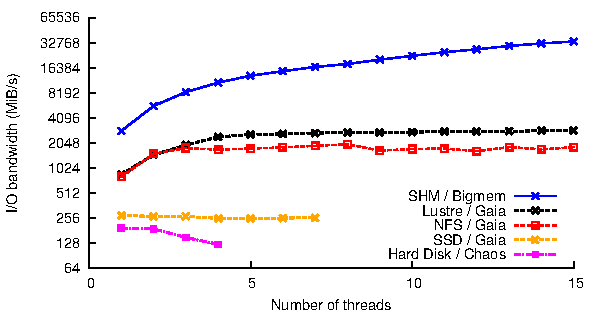
\includegraphics[width=0.9\textwidth]{iorun_read.pdf}}
      \only<2>{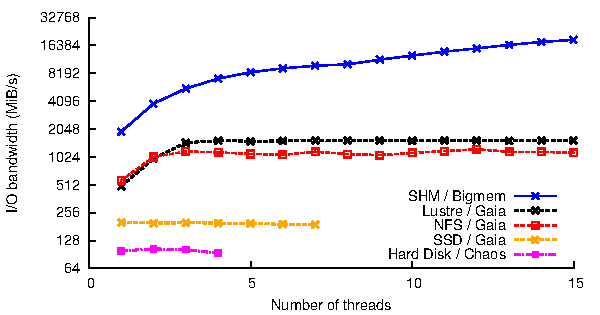
\includegraphics[width=0.9\textwidth]{iorun_write.pdf}}
  \end{center}

}

% .......
\frame{
  \frametitle{Speed Expectation on Data Transfer}
  \hfill \myurl{http://fasterdata.es.net/}

  \begin{itemize}
    \item How long to transfer \textbf{1 TB} of data across various speed networks?
      \begin{table}\centering\footnotesize
          \begin{tabular}{|c|l|}
              \rowcolor{lightgray}
              \hline
              \textbf{Network} & \textbf{Time}\\\hline
              \hline
              10 Mbps  & 300 hrs (12.5 days) \\
              100 Mbps & 30 hrs \\
              1 Gbps   & 3 hrs  \\
              10 Gbps  & 20 minutes \\
              \hline
          \end{tabular}
      \end{table}

  \end{itemize}


  % \begin{alertblock}{}
  %     \alert{\textbf{(Again)} small I/Os really \emph{kill} performances}
  % \end{alertblock}

  \begin{itemize}
    \item \textbf{(Again)} small I/Os really \emph{kill} performances
      \begin{itemize}
          \itemhook \emph{Ex}: transferring 80 TB for the backup of \texttt{ecosystem\_biology}
          \itemhook same rack, 10Gb/s. 4 weeks $\longrightarrow$ 63TB transfer...
      \end{itemize}
  \end{itemize}
}

% .......
\frame{
  \frametitle{Speed Expectation on Data Transfer}
  \hfill \myurl{http://fasterdata.es.net/}
  %\vspace{-1em}
  \begin{center}
      \only<1>{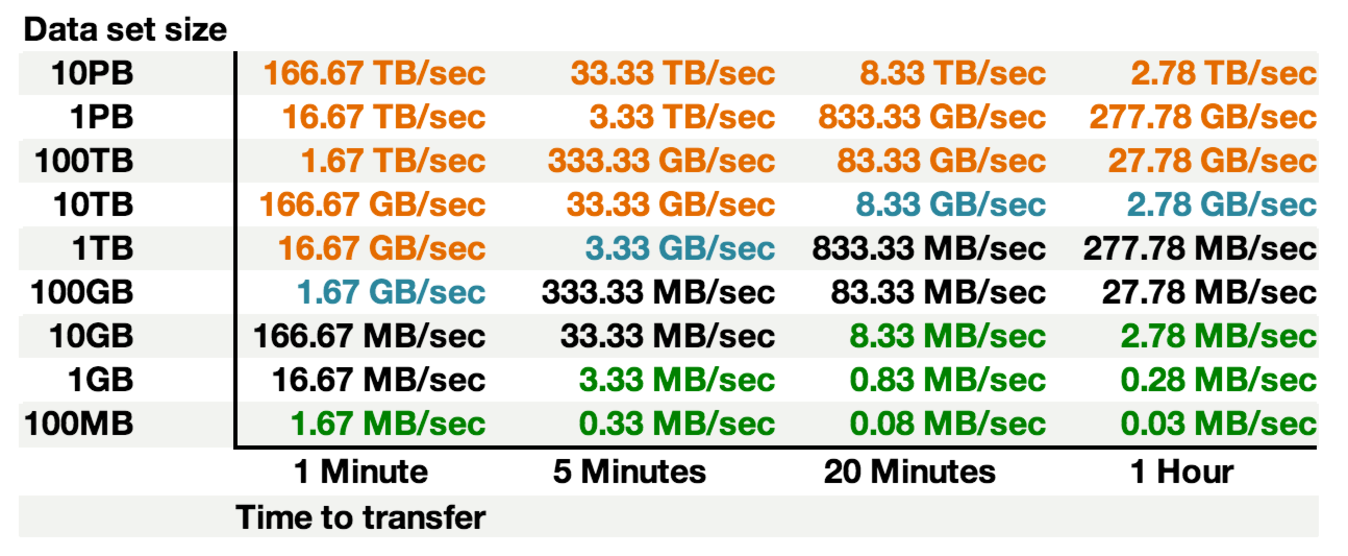
\includegraphics[scale=0.42]{fasterdata_expected_throughput_1.pdf}}
      \only<2>{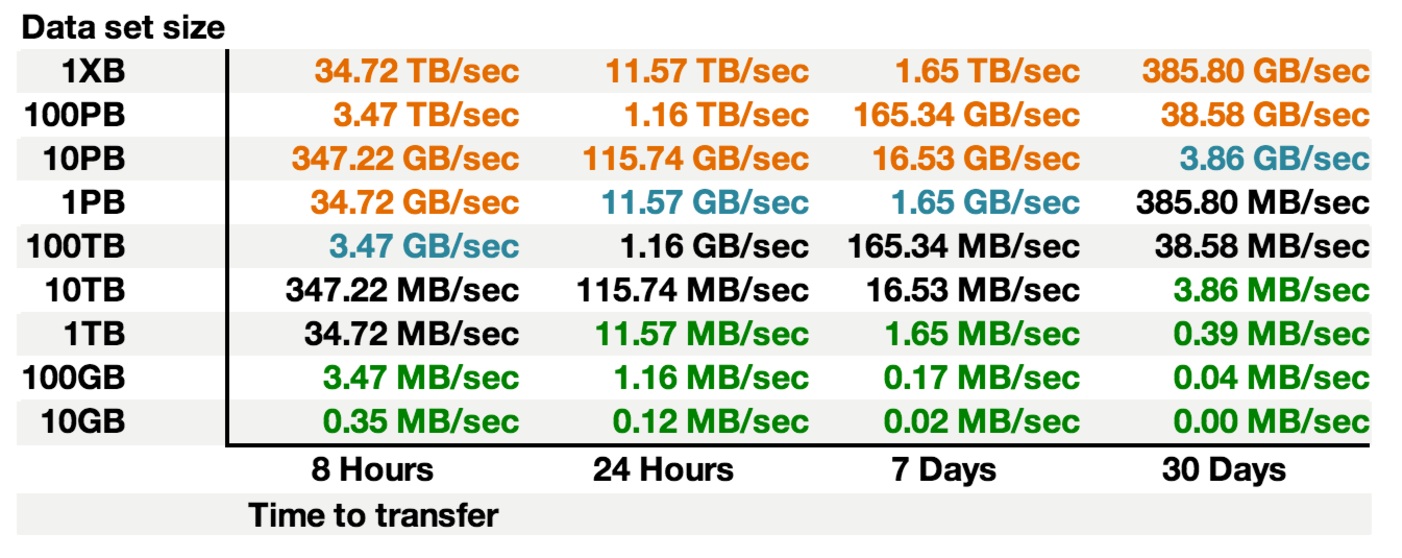
\includegraphics[scale=0.42]{fasterdata_expected_throughput_2.pdf}}
  \end{center}
  
  \hfill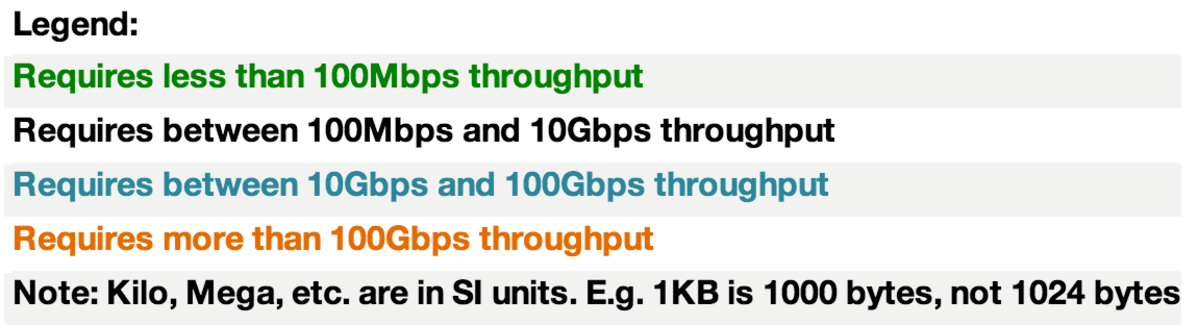
\includegraphics[scale=0.3]{fasterdata_legend.pdf}
}

\subsection{Fault Tolerance}

\begin{frame}[t]
    \frametitle{Fault Tolerance} %Last Challenges \hfill{\small for a better efficiency}}

    %\emph{Fault Tolerance}
    \begin{itemize}
      \item<+-> Cluster maintenance from time to time
      \item<+-> Reliability vs. Crash Faults in Distributed systems
        \only<2>{
          \begin{center}
              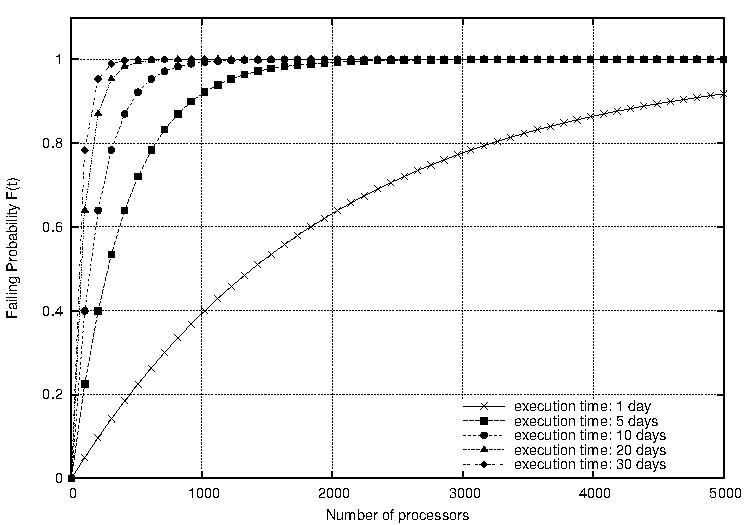
\includegraphics[width=0.5\textwidth]{proba_defaillance}
          \end{center}
        }
      \item<+-> Fault Tolerance general strategy: checkpoint/rollback
        \begin{itemize}
            \itemhook assumes a way to save the state of your program
            \itemhook hints: OAR \texttt{--signal --checkpoint --idempotent...}, BLCR
            \itemhook combine best-effort jobs with checkpointing (\myurl{http://git.io/c-dn1A})
        \end{itemize}
    \end{itemize}

\end{frame}





% ======================== END =========================
\section*{Thank you for your attention...}
\frame{
  \frametitle{Questions?}
  % ~~~~~~~~~~~~~~
  \begin{columns}[b]
    \column{0.5\textwidth}
    % \emph{Contact}\\
    {\tiny
      \emph{S\'ebastien Varrette, PhD}\\
      ~~~~ \textit{mail:} \href{mailto:sebastien.varrette@uni.lu}{sebastien.varrette@uni.lu}\\
      ~~~~ Office E-007\\
      ~~~~ Campus Kirchberg\\
      ~~~~ 6, rue Coudenhove-Kalergi\\
      ~~~~ L-1359 Luxembourg\\[1em]

      \emph{UL HPC Management Team}\\
      ~~~~ \textit{mail:} \href{mailto:hpc-sysadmins@uni.lu}{hpc-sysadmins@uni.lu}\\
      
    }
    \column{0.5\textwidth}
    % \scalebox{8}{\emph{?}}
    
\includegraphics[width=1.5in]{question.jpg}
  \end{columns}
  % Below is the table of content over 2 columns
  \vfill
  %\begin{multicols}{2}
    {\tiny \tableofcontents}
  %\end{multicols}

}

\newcounter{finalframe}
\setcounter{finalframe}{\value{framenumber}}

% %.......
% \frame{
%   \frametitle{}
%   \vfill
%   \centering \LARGE Appendix\footnote{notice the slide number below...}
%   \vfill
% }

\setcounter{framenumber}{\value{finalframe}}

\end{document}

% ~~~~~~~~~~~~~~~~~~~~~~~~~~~~~~~~~~~~~~~~~~~~~~~~~~~~~~~~~~~~~~~~
% eof
% 
% Local Variables:
% mode: latex
% mode: flyspell
% mode: visual-line
% TeX-master: "data_management.tex"
% End:
